
\input{../../2021/style/preamble4tex}
% math spaces
\ifdefined\N
\renewcommand{\N}{\mathds{N}} % N, naturals
\else \newcommand{\N}{\mathds{N}} \fi
\newcommand{\Z}{\mathds{Z}} % Z, integers
\newcommand{\Q}{\mathds{Q}} % Q, rationals
\newcommand{\R}{\mathds{R}} % R, reals
\ifdefined\C
  \renewcommand{\C}{\mathds{C}} % C, complex
\else \newcommand{\C}{\mathds{C}} \fi
\newcommand{\continuous}{\mathcal{C}} % C, space of continuous functions
\newcommand{\M}{\mathcal{M}} % machine numbers
\newcommand{\epsm}{\epsilon_m} % maximum error

% counting / finite sets
\newcommand{\setzo}{\{0, 1\}} % set 0, 1
\newcommand{\setmp}{\{-1, +1\}} % set -1, 1
\newcommand{\unitint}{[0, 1]} % unit interval

% basic math stuff
\newcommand{\xt}{\tilde x} % x tilde
\DeclareMathOperator*{\argmax}{arg\,max} % argmax
\DeclareMathOperator*{\argmin}{arg\,min} % argmin
\newcommand{\argminlim}{\mathop{\mathrm{arg\,min}}\limits} % argmax with limits
\newcommand{\argmaxlim}{\mathop{\mathrm{arg\,max}}\limits} % argmin with limits
\newcommand{\sign}{\operatorname{sign}} % sign, signum
\newcommand{\I}{\mathbb{I}} % I, indicator
\newcommand{\order}{\mathcal{O}} % O, order
\newcommand{\bigO}{\mathcal{O}} % Big-O Landau
\newcommand{\littleo}{{o}} % Little-o Landau
\newcommand{\pd}[2]{\frac{\partial{#1}}{\partial #2}} % partial derivative
\newcommand{\floorlr}[1]{\left\lfloor #1 \right\rfloor} % floor
\newcommand{\ceillr}[1]{\left\lceil #1 \right\rceil} % ceiling
\newcommand{\indep}{\perp \!\!\! \perp} % independence symbol

% sums and products
\newcommand{\sumin}{\sum\limits_{i=1}^n} % summation from i=1 to n
\newcommand{\sumim}{\sum\limits_{i=1}^m} % summation from i=1 to m
\newcommand{\sumjn}{\sum\limits_{j=1}^n} % summation from j=1 to p
\newcommand{\sumjp}{\sum\limits_{j=1}^p} % summation from j=1 to p
\newcommand{\sumik}{\sum\limits_{i=1}^k} % summation from i=1 to k
\newcommand{\sumkg}{\sum\limits_{k=1}^g} % summation from k=1 to g
\newcommand{\sumjg}{\sum\limits_{j=1}^g} % summation from j=1 to g
\newcommand{\meanin}{\frac{1}{n} \sum\limits_{i=1}^n} % mean from i=1 to n
\newcommand{\meanim}{\frac{1}{m} \sum\limits_{i=1}^m} % mean from i=1 to n
\newcommand{\meankg}{\frac{1}{g} \sum\limits_{k=1}^g} % mean from k=1 to g
\newcommand{\prodin}{\prod\limits_{i=1}^n} % product from i=1 to n
\newcommand{\prodkg}{\prod\limits_{k=1}^g} % product from k=1 to g
\newcommand{\prodjp}{\prod\limits_{j=1}^p} % product from j=1 to p

% linear algebra
\newcommand{\one}{\boldsymbol{1}} % 1, unitvector
\newcommand{\zero}{\mathbf{0}} % 0-vector
\newcommand{\id}{\boldsymbol{I}} % I, identity
\newcommand{\diag}{\operatorname{diag}} % diag, diagonal
\newcommand{\trace}{\operatorname{tr}} % tr, trace
\newcommand{\spn}{\operatorname{span}} % span
\newcommand{\scp}[2]{\left\langle #1, #2 \right\rangle} % <.,.>, scalarproduct
\newcommand{\mat}[1]{\begin{pmatrix} #1 \end{pmatrix}} % short pmatrix command
\newcommand{\Amat}{\mathbf{A}} % matrix A
\newcommand{\Deltab}{\mathbf{\Delta}} % error term for vectors

% basic probability + stats
\renewcommand{\P}{\mathds{P}} % P, probability
\newcommand{\E}{\mathds{E}} % E, expectation
\newcommand{\var}{\mathsf{Var}} % Var, variance
\newcommand{\cov}{\mathsf{Cov}} % Cov, covariance
\newcommand{\corr}{\mathsf{Corr}} % Corr, correlation
\newcommand{\normal}{\mathcal{N}} % N of the normal distribution
\newcommand{\iid}{\overset{i.i.d}{\sim}} % dist with i.i.d superscript
\newcommand{\distas}[1]{\overset{#1}{\sim}} % ... is distributed as ...

% machine learning
\newcommand{\Xspace}{\mathcal{X}} % X, input space
\newcommand{\Yspace}{\mathcal{Y}} % Y, output space
\newcommand{\Zspace}{\mathcal{Z}} % Z, space of sampled datapoints
\newcommand{\nset}{\{1, \ldots, n\}} % set from 1 to n
\newcommand{\pset}{\{1, \ldots, p\}} % set from 1 to p
\newcommand{\gset}{\{1, \ldots, g\}} % set from 1 to g
\newcommand{\Pxy}{\mathbb{P}_{xy}} % P_xy
\newcommand{\Exy}{\mathbb{E}_{xy}} % E_xy: Expectation over random variables xy
\newcommand{\xv}{\mathbf{x}} % vector x (bold)
\newcommand{\xtil}{\tilde{\mathbf{x}}} % vector x-tilde (bold)
\newcommand{\yv}{\mathbf{y}} % vector y (bold)
\newcommand{\xy}{(\xv, y)} % observation (x, y)
\newcommand{\xvec}{\left(x_1, \ldots, x_p\right)^\top} % (x1, ..., xp)
\newcommand{\Xmat}{\mathbf{X}} % Design matrix
\newcommand{\allDatasets}{\mathds{D}} % The set of all datasets
\newcommand{\allDatasetsn}{\mathds{D}_n}  % The set of all datasets of size n
\newcommand{\D}{\mathcal{D}} % D, data
\newcommand{\Dn}{\D_n} % D_n, data of size n
\newcommand{\Dtrain}{\mathcal{D}_{\text{train}}} % D_train, training set
\newcommand{\Dtest}{\mathcal{D}_{\text{test}}} % D_test, test set
\newcommand{\xyi}[1][i]{\left(\xv^{(#1)}, y^{(#1)}\right)} % (x^i, y^i), i-th observation
\newcommand{\Dset}{\left( \xyi[1], \ldots, \xyi[n]\right)} % {(x1,y1)), ..., (xn,yn)}, data
\newcommand{\defAllDatasetsn}{(\Xspace \times \Yspace)^n} % Def. of the set of all datasets of size n
\newcommand{\defAllDatasets}{\bigcup_{n \in \N}(\Xspace \times \Yspace)^n} % Def. of the set of all datasets
\newcommand{\xdat}{\left\{ \xv^{(1)}, \ldots, \xv^{(n)}\right\}} % {x1, ..., xn}, input data
\newcommand{\ydat}{\left\{ \yv^{(1)}, \ldots, \yv^{(n)}\right\}} % {y1, ..., yn}, input data
\newcommand{\yvec}{\left(y^{(1)}, \hdots, y^{(n)}\right)^\top} % (y1, ..., yn), vector of outcomes
\newcommand{\greekxi}{\xi} % Greek letter xi
\renewcommand{\xi}[1][i]{\xv^{(#1)}} % x^i, i-th observed value of x
\newcommand{\yi}[1][i]{y^{(#1)}} % y^i, i-th observed value of y
\newcommand{\xivec}{\left(x^{(i)}_1, \ldots, x^{(i)}_p\right)^\top} % (x1^i, ..., xp^i), i-th observation vector
\newcommand{\xj}{\xv_j} % x_j, j-th feature
\newcommand{\xjvec}{\left(x^{(1)}_j, \ldots, x^{(n)}_j\right)^\top} % (x^1_j, ..., x^n_j), j-th feature vector
\newcommand{\phiv}{\mathbf{\phi}} % Basis transformation function phi
\newcommand{\phixi}{\mathbf{\phi}^{(i)}} % Basis transformation of xi: phi^i := phi(xi)

%%%%%% ml - models general
\newcommand{\lamv}{\bm{\lambda}} % lambda vector, hyperconfiguration vector
\newcommand{\Lam}{\bm{\Lambda}}	 % Lambda, space of all hpos
% Inducer / Inducing algorithm
\newcommand{\preimageInducer}{\left(\defAllDatasets\right)\times\Lam} % Set of all datasets times the hyperparameter space
\newcommand{\preimageInducerShort}{\allDatasets\times\Lam} % Set of all datasets times the hyperparameter space
% Inducer / Inducing algorithm
\newcommand{\ind}{\mathcal{I}} % Inducer, inducing algorithm, learning algorithm

% continuous prediction function f
\newcommand{\ftrue}{f_{\text{true}}}  % True underlying function (if a statistical model is assumed)
\newcommand{\ftruex}{\ftrue(\xv)} % True underlying function (if a statistical model is assumed)
\newcommand{\fx}{f(\xv)} % f(x), continuous prediction function
\newcommand{\fdomains}{f: \Xspace \rightarrow \R^g} % f with domain and co-domain
\newcommand{\Hspace}{\mathcal{H}} % hypothesis space where f is from
\newcommand{\fbayes}{f^{\ast}} % Bayes-optimal model
\newcommand{\fxbayes}{f^{\ast}(\xv)} % Bayes-optimal model
\newcommand{\fkx}[1][k]{f_{#1}(\xv)} % f_j(x), discriminant component function
\newcommand{\fh}{\hat{f}} % f hat, estimated prediction function
\newcommand{\fxh}{\fh(\xv)} % fhat(x)
\newcommand{\fxt}{f(\xv ~|~ \thetav)} % f(x | theta)
\newcommand{\fxi}{f\left(\xv^{(i)}\right)} % f(x^(i))
\newcommand{\fxih}{\hat{f}\left(\xv^{(i)}\right)} % f(x^(i))
\newcommand{\fxit}{f\left(\xv^{(i)} ~|~ \thetav\right)} % f(x^(i) | theta)
\newcommand{\fhD}{\fh_{\D}} % fhat_D, estimate of f based on D
\newcommand{\fhDtrain}{\fh_{\Dtrain}} % fhat_Dtrain, estimate of f based on D
\newcommand{\fhDnlam}{\fh_{\Dn, \lamv}} %model learned on Dn with hp lambda
\newcommand{\fhDlam}{\fh_{\D, \lamv}} %model learned on D with hp lambda
\newcommand{\fhDnlams}{\fh_{\Dn, \lamv^\ast}} %model learned on Dn with optimal hp lambda
\newcommand{\fhDlams}{\fh_{\D, \lamv^\ast}} %model learned on D with optimal hp lambda

% discrete prediction function h
\newcommand{\hx}{h(\xv)} % h(x), discrete prediction function
\newcommand{\hh}{\hat{h}} % h hat
\newcommand{\hxh}{\hat{h}(\xv)} % hhat(x)
\newcommand{\hxt}{h(\xv | \thetav)} % h(x | theta)
\newcommand{\hxi}{h\left(\xi\right)} % h(x^(i))
\newcommand{\hxit}{h\left(\xi ~|~ \thetav\right)} % h(x^(i) | theta)
\newcommand{\hbayes}{h^{\ast}} % Bayes-optimal classification model
\newcommand{\hxbayes}{h^{\ast}(\xv)} % Bayes-optimal classification model

% yhat
\newcommand{\yh}{\hat{y}} % yhat for prediction of target
\newcommand{\yih}{\hat{y}^{(i)}} % yhat^(i) for prediction of ith targiet
\newcommand{\resi}{\yi- \yih}

% theta
\newcommand{\thetah}{\hat{\theta}} % theta hat
\newcommand{\thetav}{\bm{\theta}} % theta vector
\newcommand{\thetavh}{\bm{\hat\theta}} % theta vector hat
\newcommand{\thetat}[1][t]{\thetav^{[#1]}} % theta^[t] in optimization
\newcommand{\thetatn}[1][t]{\thetav^{[#1 +1]}} % theta^[t+1] in optimization
\newcommand{\thetahDnlam}{\thetavh_{\Dn, \lamv}} %theta learned on Dn with hp lambda
\newcommand{\thetahDlam}{\thetavh_{\D, \lamv}} %theta learned on D with hp lambda
\newcommand{\mint}{\min_{\thetav \in \Theta}} % min problem theta
\newcommand{\argmint}{\argmin_{\thetav \in \Theta}} % argmin theta

% densities + probabilities
% pdf of x
\newcommand{\pdf}{p} % p
\newcommand{\pdfx}{p(\xv)} % p(x)
\newcommand{\pixt}{\pi(\xv~|~ \thetav)} % pi(x|theta), pdf of x given theta
\newcommand{\pixit}[1][i]{\pi\left(\xi[#1] ~|~ \thetav\right)} % pi(x^i|theta), pdf of x given theta
\newcommand{\pixii}[1][i]{\pi\left(\xi[#1]\right)} % pi(x^i), pdf of i-th x

% pdf of (x, y)
\newcommand{\pdfxy}{p(\xv,y)} % p(x, y)
\newcommand{\pdfxyt}{p(\xv, y ~|~ \thetav)} % p(x, y | theta)
\newcommand{\pdfxyit}{p\left(\xi, \yi ~|~ \thetav\right)} % p(x^(i), y^(i) | theta)

% pdf of x given y
\newcommand{\pdfxyk}[1][k]{p(\xv | y= #1)} % p(x | y = k)
\newcommand{\lpdfxyk}[1][k]{\log p(\xv | y= #1)} % log p(x | y = k)
\newcommand{\pdfxiyk}[1][k]{p\left(\xi | y= #1 \right)} % p(x^i | y = k)

% prior probabilities
\newcommand{\pik}[1][k]{\pi_{#1}} % pi_k, prior
\newcommand{\lpik}[1][k]{\log \pi_{#1}} % log pi_k, log of the prior
\newcommand{\pit}{\pi(\thetav)} % Prior probability of parameter theta

% posterior probabilities
\newcommand{\post}{\P(y = 1 ~|~ \xv)} % P(y = 1 | x), post. prob for y=1
\newcommand{\postk}[1][k]{\P(y = #1 ~|~ \xv)} % P(y = k | y), post. prob for y=k
\newcommand{\pidomains}{\pi: \Xspace \rightarrow \unitint} % pi with domain and co-domain
\newcommand{\pibayes}{\pi^{\ast}} % Bayes-optimal classification model
\newcommand{\pixbayes}{\pi^{\ast}(\xv)} % Bayes-optimal classification model
\newcommand{\pix}{\pi(\xv)} % pi(x), P(y = 1 | x)
\newcommand{\piv}{\bm{\pi}} % pi, bold, as vector
\newcommand{\pikx}[1][k]{\pi_{#1}(\xv)} % pi_k(x), P(y = k | x)
\newcommand{\pikxt}[1][k]{\pi_{#1}(\xv ~|~ \thetav)} % pi_k(x | theta), P(y = k | x, theta)
\newcommand{\pixh}{\hat \pi(\xv)} % pi(x) hat, P(y = 1 | x) hat
\newcommand{\pikxh}[1][k]{\hat \pi_{#1}(\xv)} % pi_k(x) hat, P(y = k | x) hat
\newcommand{\pixih}{\hat \pi(\xi)} % pi(x^(i)) with hat
\newcommand{\pikxih}[1][k]{\hat \pi_{#1}(\xi)} % pi_k(x^(i)) with hat
\newcommand{\pdfygxt}{p(y ~|~\xv, \thetav)} % p(y | x, theta)
\newcommand{\pdfyigxit}{p\left(\yi ~|~\xi, \thetav\right)} % p(y^i |x^i, theta)
\newcommand{\lpdfygxt}{\log \pdfygxt } % log p(y | x, theta)
\newcommand{\lpdfyigxit}{\log \pdfyigxit} % log p(y^i |x^i, theta)

% probababilistic
\newcommand{\bayesrulek}[1][k]{\frac{\P(\xv | y= #1) \P(y= #1)}{\P(\xv)}} % Bayes rule
\newcommand{\muk}{\bm{\mu_k}} % mean vector of class-k Gaussian (discr analysis)

% residual and margin
\newcommand{\eps}{\epsilon} % residual, stochastic
\newcommand{\epsv}{\bm{\epsilon}} % residual, stochastic, as vector
\newcommand{\epsi}{\epsilon^{(i)}} % epsilon^i, residual, stochastic
\newcommand{\epsh}{\hat{\epsilon}} % residual, estimated
\newcommand{\epsvh}{\hat{\epsv}} % residual, estimated, vector
\newcommand{\yf}{y \fx} % y f(x), margin
\newcommand{\yfi}{\yi \fxi} % y^i f(x^i), margin
\newcommand{\Sigmah}{\hat \Sigma} % estimated covariance matrix
\newcommand{\Sigmahj}{\hat \Sigma_j} % estimated covariance matrix for the j-th class

% ml - loss, risk, likelihood
\newcommand{\Lyf}{L\left(y, f\right)} % L(y, f), loss function
\newcommand{\Lypi}{L\left(y, \pi\right)} % L(y, pi), loss function
\newcommand{\Lxy}{L\left(y, \fx\right)} % L(y, f(x)), loss function
\newcommand{\Lxyi}{L\left(\yi, \fxi\right)} % loss of observation
\newcommand{\Lxyt}{L\left(y, \fxt\right)} % loss with f parameterized
\newcommand{\Lxyit}{L\left(\yi, \fxit\right)} % loss of observation with f parameterized
\newcommand{\Lxym}{L\left(\yi, f\left(\bm{\tilde{x}}^{(i)} ~|~ \thetav\right)\right)} % loss of observation with f parameterized
\newcommand{\Lpixy}{L\left(y, \pix\right)} % loss in classification
\newcommand{\Lpiv}{L\left(y, \piv\right)} % loss in classification
\newcommand{\Lpixyi}{L\left(\yi, \pixii\right)} % loss of observation in classification
\newcommand{\Lpixyt}{L\left(y, \pixt\right)} % loss with pi parameterized
\newcommand{\Lpixyit}{L\left(\yi, \pixit\right)} % loss of observation with pi parameterized
\newcommand{\Lhxy}{L\left(y, \hx\right)} % L(y, h(x)), loss function on discrete classes
\newcommand{\Lr}{L\left(r\right)} % L(r), loss defined on residual (reg) / margin (classif)
\newcommand{\lone}{|y - \fx|} % L1 loss
\newcommand{\ltwo}{\left(y - \fx\right)^2} % L2 loss
\newcommand{\lbernoullimp}{\ln(1 + \exp(-y \cdot \fx))} % Bernoulli loss for -1, +1 encoding
\newcommand{\lbernoullizo}{- y \cdot \fx + \log(1 + \exp(\fx))} % Bernoulli loss for 0, 1 encoding
\newcommand{\lcrossent}{- y \log \left(\pix\right) - (1 - y) \log \left(1 - \pix\right)} % cross-entropy loss
\newcommand{\lbrier}{\left(\pix - y \right)^2} % Brier score
\newcommand{\risk}{\mathcal{R}} % R, risk
\newcommand{\riskbayes}{\mathcal{R}^\ast}
\newcommand{\riskf}{\risk(f)} % R(f), risk
\newcommand{\riskdef}{\E_{y|\xv}\left(\Lxy \right)} % risk def (expected loss)
\newcommand{\riskt}{\mathcal{R}(\thetav)} % R(theta), risk
\newcommand{\riske}{\mathcal{R}_{\text{emp}}} % R_emp, empirical risk w/o factor 1 / n
\newcommand{\riskeb}{\bar{\mathcal{R}}_{\text{emp}}} % R_emp, empirical risk w/ factor 1 / n
\newcommand{\riskef}{\riske(f)} % R_emp(f)
\newcommand{\risket}{\mathcal{R}_{\text{emp}}(\thetav)} % R_emp(theta)
\newcommand{\riskr}{\mathcal{R}_{\text{reg}}} % R_reg, regularized risk
\newcommand{\riskrt}{\mathcal{R}_{\text{reg}}(\thetav)} % R_reg(theta)
\newcommand{\riskrf}{\riskr(f)} % R_reg(f)
\newcommand{\riskrth}{\hat{\mathcal{R}}_{\text{reg}}(\thetav)} % hat R_reg(theta)
\newcommand{\risketh}{\hat{\mathcal{R}}_{\text{emp}}(\thetav)} % hat R_emp(theta)
\newcommand{\LL}{\mathcal{L}} % L, likelihood
\newcommand{\LLt}{\mathcal{L}(\thetav)} % L(theta), likelihood
\newcommand{\LLtx}{\mathcal{L}(\thetav | \xv)} % L(theta|x), likelihood
\newcommand{\logl}{\ell} % l, log-likelihood
\newcommand{\loglt}{\logl(\thetav)} % l(theta), log-likelihood
\newcommand{\logltx}{\logl(\thetav | \xv)} % l(theta|x), log-likelihood
\newcommand{\errtrain}{\text{err}_{\text{train}}} % training error
\newcommand{\errtest}{\text{err}_{\text{test}}} % test error
\newcommand{\errexp}{\overline{\text{err}_{\text{test}}}} % avg training error

% lm
\newcommand{\thx}{\thetav^\top \xv} % linear model
\newcommand{\olsest}{(\Xmat^\top \Xmat)^{-1} \Xmat^\top \yv} % OLS estimator in LM


\begin{document}

\lecturechapter{12}{Advanced ROC Analysis}
\lecture{Fortgeschrittene Computerintensive Methoden}

%
% \begin{vbframe}{Prediction Types}
% %Appropriate performance measures are available for each prediction type:
% Depending on the prediction type of (binary) classifiers, some performance measures are more appropriate than others:
%
% \begin{itemize}
% \item \textbf{Discrete classes:} confusion matrix and any measure based on it, e.g., (balanced) accuracy, precision, recall/TPR, FPR, F1, ...
% \item \textbf{Scores / Probabilities:}
% \begin{itemize}
% \item Summary measures: AUC, MAE, Brier Score (L2 Loss), ...
% \item Visual measures: ROC curves, precision-recall curves, cost curves, calibration plot, ...
% \end{itemize}
% \end{itemize}
%
% %Discrete classifiers, scoring classifiers, and probabilistic classifiers produce different types of predictions:
%
% \begin{figure}[!htb]
% \centering
% \includegraphics[width=0.5\textwidth]{figure_man/predtype.pdf}
% \end{figure}
% \end{vbframe}

\begin{vbframe}{Recall: ROC curve and AUC}
\small
  \begin{itemize}
  \item Points in the ROC space visualize the true positive rate (TPR) and false positive rate (FPR) of a classifier that predicts discrete classes.
  %\item The best classifier lies on the top-left corner.
  %\item A random classifier results in a diagonal line (baseline).
  %\item Each point on the baseline refers to different proportions for predicting the positive class "1".
  \item For classifiers that predict probabilities/scores we can use different thresholds to convert their predictions to discrete classes.
\item For each possible threshold we can draw a point in the ROC space. Connecting these points yields a ROC curve.
\item The area under the ROC curve (AUC $\in [0, 1]$) is a scalar measure to assess the predicted probabilities/scores of a classifier.
\end{itemize}



% \framebreak
%
% \begin{itemize}
%
% \item The area under the ROC curve (AUC $\in [0, 1]$) is a scalar measure to assess the predicted probabilities/scores of a classifier:
%   \begin{itemize}
%     \item AUC =   1: Perfect classifier, for which all positives are ranked higher than all negatives.
%     \item AUC = 0.5: Randomly ordered.
%     \item AUC =   0: All negatives are ranked higher than all positives.
%   \end{itemize}
% \end{itemize}
%

\begin{center}
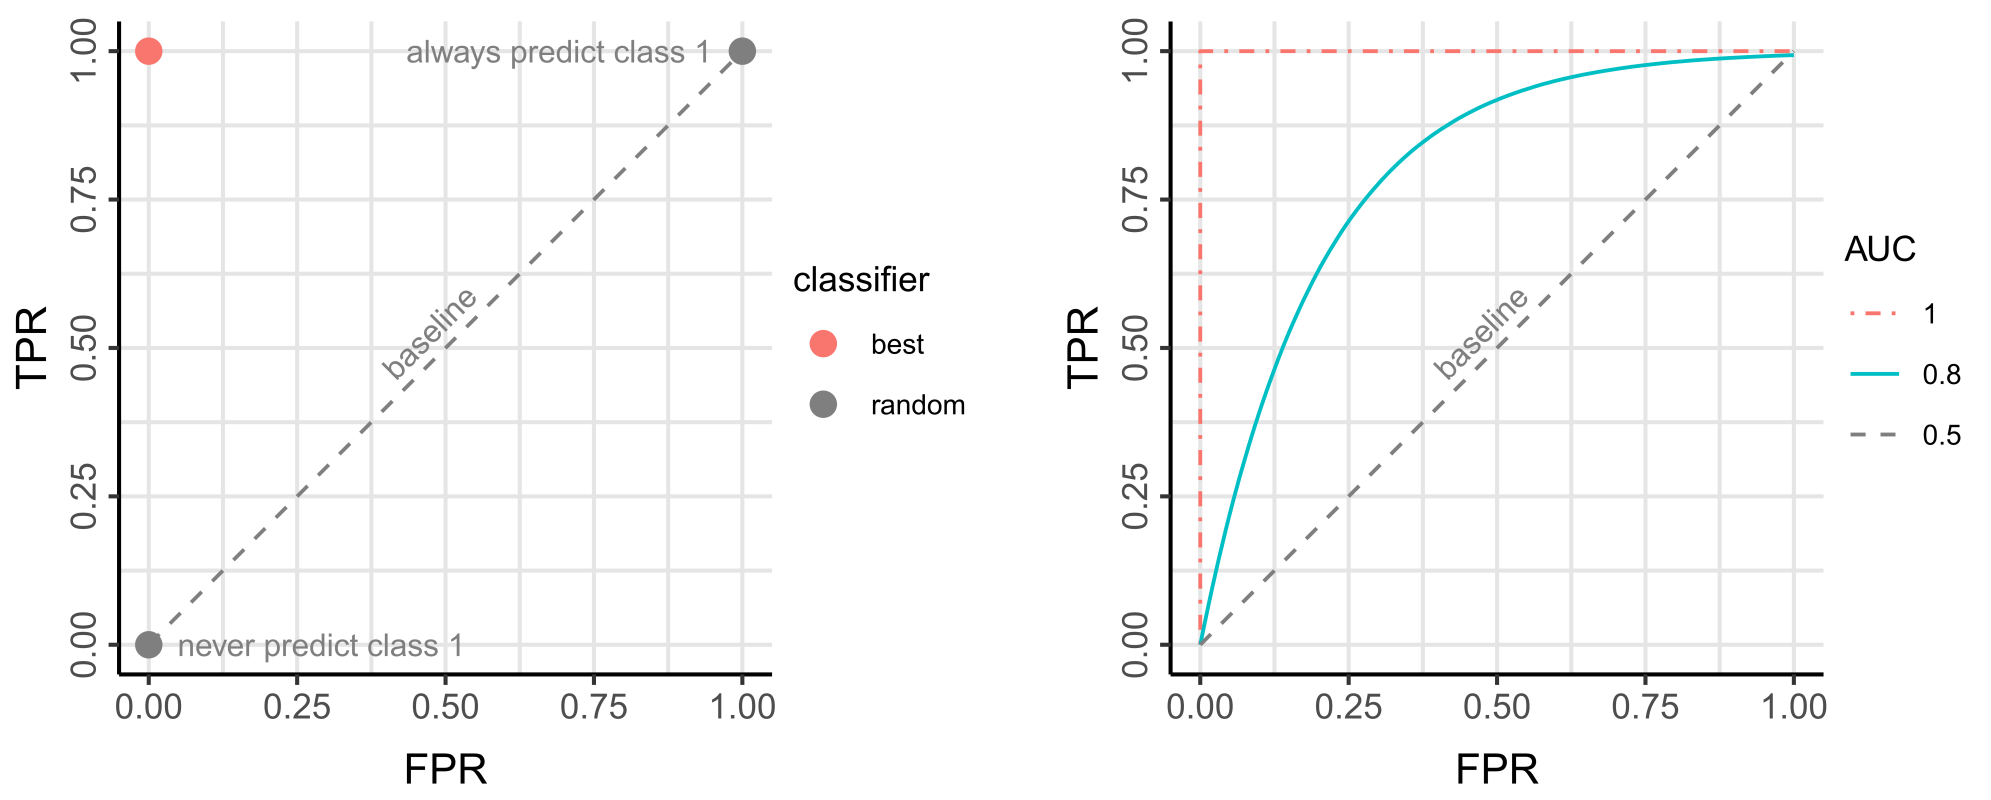
\includegraphics[width=0.7\textwidth]{figure_man/roc.png}
\end{center}

\end{vbframe}

% \begin{vbframe}{Advanced ROC Analysis}
%   \begin{itemize}
%     \item We introduce iso-accuracy lines, which allow to directly read off the accuracy/misclassification error from points in a ROC curve.
%     \item For a specific class distribution, iso-accuracy lines can be used to find the best
%   \end{itemize}
% \end{vbframe}


\begin{vbframe}{ISO-Accuracy Lines}

\normalsize

Iso-accuracy lines allow to directly read off the resulting accuracy of points in the ROC space.
This is possible because of the relationship between accuracy ($acc$) and FPR/TPR:

\begin{minipage}{0.6\textwidth}
\begin{align*}
 \text{acc}
 &= \cfrac{\text{\#TP} + \text{\#TN}}{n} = \cfrac{\text{\#TP} +  \nn - \text{\#FP}}{n} \\
 &=
 %\cfrac{\text{\#TP}}{\np} \cdot \cfrac{\np}{n} + \cfrac{\nn - \text{\#FP}}{n} \\
    \cfrac{\np}{n} \cdot \cfrac{\text{\#TP}}{\np}  +
    \cfrac{\nn}{n} \cdot \left(1 - \cfrac{\text{\#FP}}{\nn} \right)\\
    %\cfrac{\nn}{n} - \cfrac{\text{\#FP}}{\nn} \cdot \cfrac{\nn}{n} \\
    & = \rp \cdot \text{TPR}  + \rn \cdot (1 - \text{FPR})
\end{align*}
\end{minipage}
\begin{minipage}{0.375\textwidth}  %%<--- here
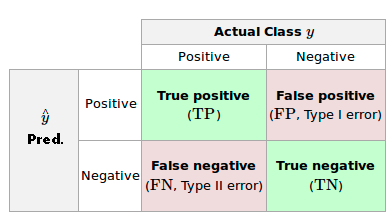
\includegraphics[width=\textwidth]{figure_man/roc-confmatrix1.png}
\end{minipage}

\lz Here, $n$ is the number of observations,
\begin{itemize}
  \item $\rn = \tfrac{\nn}{n}$ and $\rp = \tfrac{\np}{n}$ the fractions of negative and positive observations, respectively.
\end{itemize}
\end{vbframe}


\begin{vbframe}{ISO-Accuracy Lines}
We can rewrite this equation to obtain a so-called iso-accuracy line that can be plotted into the ROC space:
$$\text{TPR} =  \cfrac{\rn}{\rp}
\cdot \text{FPR} + \cfrac{\text{acc} -
\rn}{\rp}.$$

Properties:
\begin{itemize}
  \item The ratio $\tfrac{\rn}{\rp} = \tfrac{\nn}{\np}$ determines the slope of the iso-accuracy line (changing this ratio yields lines with different slopes).
  \item Different accuracies yield parallel lines with the same slope because $acc$ is included in the intercept.
  \item For a given ratio $\tfrac{\nn}{\np}$, "higher" lines are  better in terms of $acc$.
  \item Thus, we can use iso-accuracy lines to determine the "best classifier" w.r.t. $acc$.
\end{itemize}
\end{vbframe}


\begin{vbframe}{ISO Accuracy Lines}
To directly read off the accuracy of a classifier, we have to

\begin{itemize}
\item determine the slope of the lines by computing the ratio $\tfrac{\nn}{\np}$,
\item find the intersection between the descending diagonal line (blue) and the iso-accuracy line (red) that passes through the classifier's $(\text{TPR}, \text{FPR})$-point in the ROC space, and
\item project this point to the \text{TPR} axis to obtain the classifier's accuracy.
\end{itemize}

\begin{center}
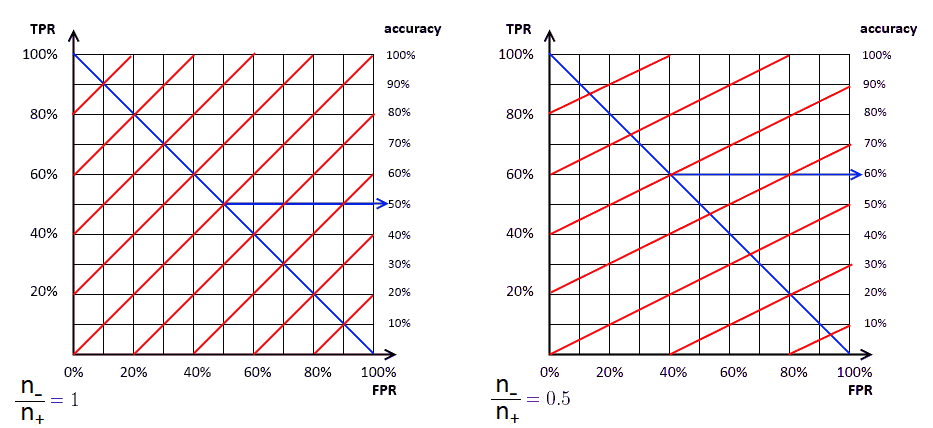
\includegraphics[width=0.85\textwidth]{figure_man/iso_lines.png}
\end{center}
\end{vbframe}

\begin{vbframe}{ISO Accuracy Lines}
To derive this mathematically, consider the following equations:
\begin{itemize}
 \item[(1)] Iso-accuracy line: $\text{TPR} =  \tfrac{\rn}{\rp}
\cdot \text{FPR} + \tfrac{\text{acc} -
\rn}{\rp}$
 \item[(2)] Descending diagonal: $\text{TPR} = 1-\text{FPR} \; \Leftrightarrow \text{FPR} = 1-\text{TPR}$
\end{itemize}

\lz At the intersection between these lines, we can plug \textbf{(2)} into \textbf{(1)}: % $\text{FPR} = 1-\text{TPR}$:
\begin{align*}
 \text{TPR} &= \tfrac{\rn}{\rp} \cdot (1-\text{TPR}) + \tfrac{\text{acc} -
 \rn}{\rp}
 %= \tfrac{\rn}{\rp} - \tfrac{\rn}{\rp} \cdot \text{TPR} + \tfrac{\text{acc} - \rn}{\rp} \\
 %&= \tfrac{\text{acc}}{\rp} - \tfrac{\rn \cdot \text{TPR}}{\rp}
 = \tfrac{\text{acc} -\rn \cdot \text{TPR}}{\rp}.
 \end{align*}

Since $\rp + \rn = 1$, this is equivalent to:
\begin{align*}
 \rp \cdot \text{TPR} + \rn \cdot \text{TPR} &= \text{acc} \\
 \Leftrightarrow \hspace{2cm} \text{TPR} &= \text{acc}
 \end{align*}

$\Rightarrow$ At the intersection between the descending diagonal line and the iso-accuracy line, the achieved accuracy is equal to the TPR, i.e., we can directly read off the $acc$ from the TPR-axis of the ROC curve.
\end{vbframe}

% \begin{vbframe}{ROC Convex Hull}
%
% Suppose we have 5 classifiers $h_1, h_2, ..., h_5$
%
% \begin{itemize}
% \item   We calculate $\text{FPR}$ and $\text{TPR}$ for each and plot them on one plot.
% \item   Each classifier is a single point in the ROC space.
% \end{itemize}
%
% \begin{center}
% 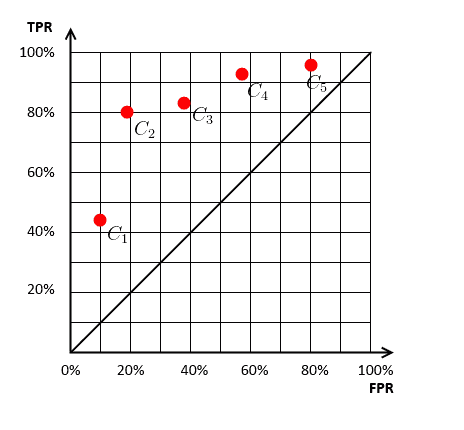
\includegraphics[width=0.5\textwidth]{figure_man/roc-plot-classifiers.png}
% \end{center}
%
% \end{vbframe}

% \begin{vbframe}{ROC Convex Hull}
% %We can try to find classifiers that achieve the best $FPR$ and $TPR$.
%
% \begin{itemize}
%   \item The classifiers $C_1, C_2, ..., C_5$ are points in the ROC space.
%   \item  %By the \href{http://0agr.ru/wiki/index.php/Dominance}{dominance} principle, we have the following Pareto frontier (the "ROC convex hull").
%   Classifiers on the convex hull \enquote{dominate} those below it (e.g. $C_3$).
%   \item Classifiers below this hull are suboptimal in this sense: they have either lower TPR \textbf{or} higher FPR.
%   \item Dominating classifiers achieve the highest total accuracy for a given class distribution (can be derived with iso-accuracy lines).
% \end{itemize}
% \hspace*{\fill}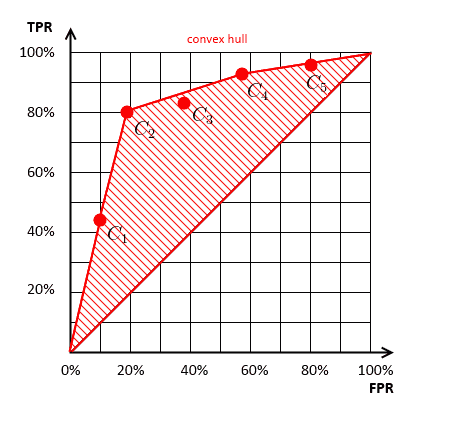
\includegraphics[width=0.4\textwidth]{figure_man/roc-convex-hull.png}\hspace*{\fill}
% % this example sucks because C3 is not clearly worse (it has better tpr than C2 and C1)
% \end{vbframe}

\begin{vbframe}{ISO Accuracy Lines}
%Each line segment of the ROC convex hull is an iso-accuracy line for a particular class distribution (slope) and accuracy.
All classifiers lying on an iso-accuracy line have the same accuracy for a particular class distribution which is determined by the slope of the iso-accuracy line:

\begin{itemize}
  \item If $\tfrac{\nn}{\np} > 1$ (class distribution with more negative observations), the slope is steeper than the diagonal line.
  % \begin{itemize}
  %   \item   The slope is steeper than the diagonal line.
  %   \item   Classifier to the left (less false positives) is more accurate.
  % \end{itemize}
  \item If $\tfrac{\nn}{\np} < 1$ (class distribution with more positive observations), the slope is flatter than the diagonal line.
  % \begin{itemize}
  %   \item   The slope is flatter than the diagonal line.
  %   \item   Classifier to the right (more false positives) is more accurate.
  % \end{itemize}
\end{itemize}
%Each classifier on the convex hull is optimal w.r.t. accuracy for a specific class distribution.

\lz
Iso-accuracy lines can therefore be used to find the "best classifier" with highest accuracy for a given class distribution $\tfrac{\nn}{\np}$:
\begin{enumerate}
  \item Compute the ratio $\tfrac{\nn}{\np}$ (i.e., the slope of the iso-accuracy line).
  \item Find the classifier (i.e., point on the ROC space) that touches the highest iso-accuracy line (i.e., the line whose intersection with the descending diagonal results in the highest accuracy).
  %\item Find highest iso-accuracy line that touches the classifier (i.e., point on the ROC space).
  %\item Use the classifier that touches the iso-accuracy line at its highest accuracy.
  %Project the intersection of the iso-accuracy line and the descending diagonal line onto the TPR-axis to obtain the classifiers accuracy.
\end{enumerate}

%
% \begin{columns}[c]
% \begin{column}{0.55\textwidth}
% 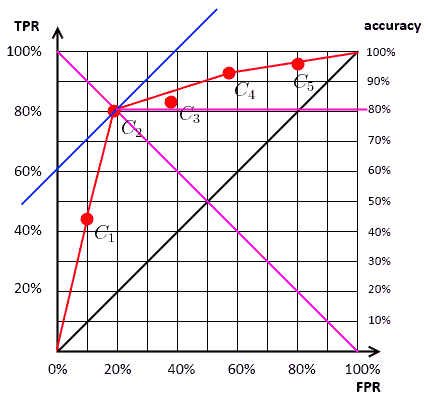
\includegraphics[width=\textwidth]{figure_man/roc-convex-hull-best-acc-1.png}
% \end{column}
% \begin{column}{0.45\textwidth}  %%<--- here
% \begin{itemize}
%   \item Class distribution: $\tfrac{\nn}{\np} = \tfrac{1}{1}$
%   \item Best classifier: $C_2$
%   \item Accuracy: $acc \approx 81 \%$
% \end{itemize}
% \end{column}
% \end{columns}
\end{vbframe}

\begin{vbframe}{Classifier with Highest Accuracy}
\textbf{Example}: Choose the best classifier among $h_1, \dots, h_5$ with highest accuracy for a specific class distribution $\tfrac{\nn}{\np}$:
\begin{columns}[c]
\begin{column}{0.475\textwidth}
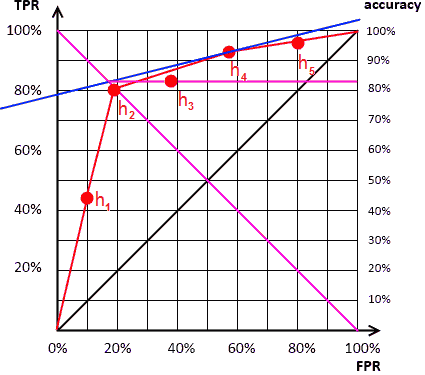
\includegraphics[width=\textwidth]{figure_man/roc-convex-hull-best-acc-2.png}
%\vspace{-15pt}
\begin{itemize}
  \item Class distribution: $\tfrac{\nn}{\np} = \tfrac{1}{4}$
  \item Best classifier: $h_4$
  \item Accuracy: $acc \approx 83 \%$
\end{itemize}
\end{column}
\vrule{}
\begin{column}{0.475\textwidth}  %%<--- here
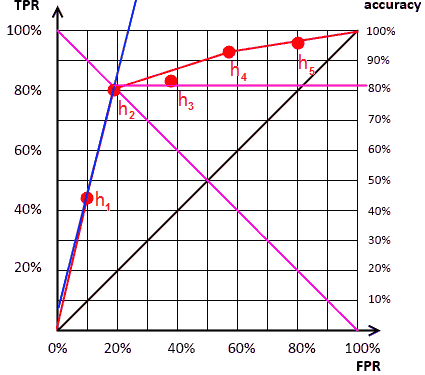
\includegraphics[width=\textwidth]{figure_man/roc-convex-hull-best-acc-3.png}
%\vspace{-15pt}
\begin{itemize}
  \item Class distribution: $\tfrac{\nn}{\np} = \tfrac{4}{1}$
  \item Best classifier: $h_2$
  \item Accuracy: $acc \approx 81 \%$
\end{itemize}
\end{column}
\end{columns}
\end{vbframe}


\begin{vbframe}{Classifier with Highest Accuracy}

For \textbf{scoring classifiers}, the classifier with highest accuracy depends on the probability threshold.

\begin{itemize}
  \item The iso-accuracy procedure is applicable to scoring classifiers analogously.
  \item Instead of different discrete classifiers (i.e., points in the ROC space), we have a ROC curve where each point in the ROC space refers to a probability threshold of a single classifier.
  \item The optimal threshold w.r.t. accuracy is the "highest tangent" of the respective ROC curve having slope $\tfrac{\nn}{\np}$ (i.e., the iso-accuracy line with highest accuracy).
\end{itemize}
\end{vbframe}

\begin{vbframe}{Classifier with Highest Accuracy}
\textbf{Example}: Find the optimal threshold of a scoring classifier w.r.t. accuracy for a given class distribution $\tfrac{\nn}{\np}$:

\begin{center}
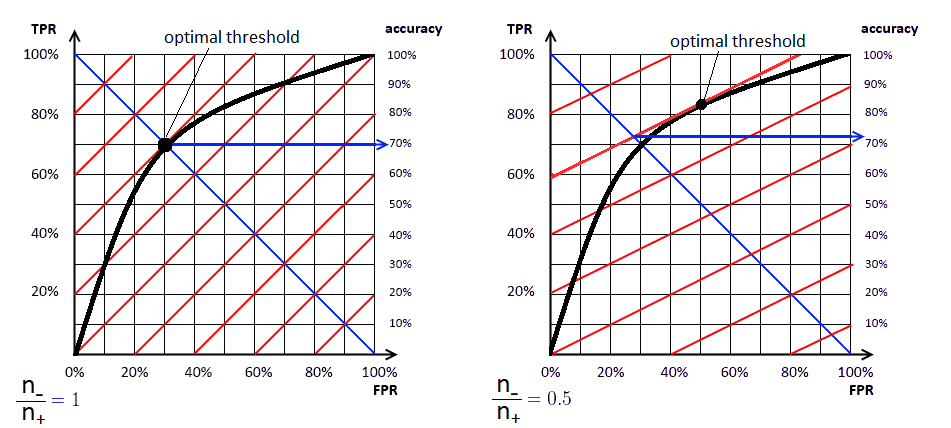
\includegraphics[width=\textwidth]{figure_man/iso_lines_2.png}
\end{center}
\end{vbframe}

\begin{vbframe}{Incorporating Costs}

\begin{itemize}
\item Analogously, iso-error lines are derived based on the relationship between the misclassification error and the TPR / FPR:
\begin{equation*}
error = \rp \cdot (1-\text{TPR}) + \rn \cdot \text{FPR}.
\end{equation*}
\item Iso-error lines have the same slope (i.e., $\tfrac{\rn}{\rp}=\tfrac{\nn}{\np}$) and result in the same decisions w.r.t. the "best classifier" as iso-accuracy lines. %but a different intercept as iso-accuracy lines.
\item Incorporating misclassification costs for false positives ($cost_{FP}$) and false negatives ($cost_{FN}$) yields the cost measure $costs$:
\begin{equation*}
costs = \rp \cdot (1-\text{TPR}) \cdot cost_{FN} + \rn \cdot \text{FPR} \cdot cost_{FP}.
\end{equation*}
\item Analogously, we can derive iso-cost lines using $costs$.
\item The slope of an iso-cost line is $\tfrac{\rn \cdot cost_{FP}}{\rp \cdot cost_{FN}} = \tfrac{\nn \cdot cost_{FP}}{\np \cdot cost_{FN}}$.
Thus, they can be used to find the "best classifier" w.r.t. $costs$ for different cost ratios and different class distributions.
%That is, we can vary not only the class distribution $\tfrac{\nn}{\np}$ but also use different costs to find the "best classifier" w.r.t. costs $C$.
%, where $cost_{FP}$ denotes the cost of predicting a positive when the sample is actually negative (and vice versa for $cost_{FN}$).
\end{itemize}

% source: http://people.cs.bris.ac.uk/~flach/ICML04tutorial/ROCtutorialPartI.pdf
\end{vbframe}


\begin{vbframe}{Incorporating Costs}
\begin{center}
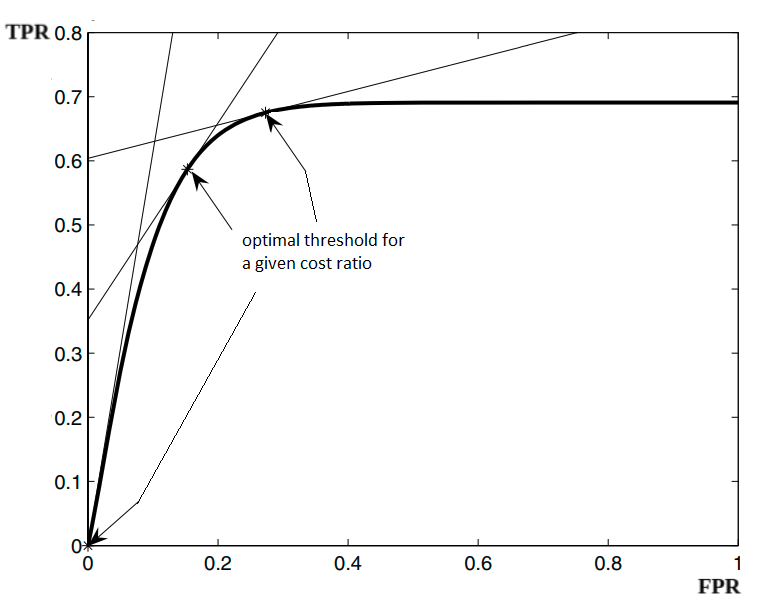
\includegraphics[width=0.45\textwidth]{figure_man/iso-cost.png}
\end{center}

\vspace{-0.5cm}
\begin{itemize}
  \item The figure shows the ROC curve of a scoring classifier where each point on the curve refers to a different probability threshold.
  \item The different iso-cost lines are tangents to the ROC curve for different cost ratios $\tfrac{cost_{FP}}{cost_{FN}}$ (but the same class distribution).
  \item The touch point between the tangents and the ROC curve refers to the optimal threshold for different cost ratios yielding the best value for $costs$.
  %\item The slope of the optimal iso line decreases with an increasing cost ratio.
  %\item In contrast to iso-accuracy lines where the $acc$ can be directly read off from the $TPR$-axis (since $TPR = acc$), the exact value of $costs$ cannot be directly read off from the $TPR$-axis.
\end{itemize}


% source: http://citeseerx.ist.psu.edu/viewdoc/download?doi=10.1.1.324.173&rep=rep1&type=pdf
\end{vbframe}

% \begin{itemize}
% \item For classifiers that predict probabilities/scores, we can use different thresholds to convert the predictions to discrete classes.
% \item To produce a ROC curve, we iterate through all possible thresholds, draw a point in the ROC space (FPR, TPR) for the resulting classifier, and connect these points.
% \item The AUC ($\in [0, 1]$) is a scalar measure to assess the predicted probabilities/scores of a classifier:
%   \begin{itemize}
%     \item AUC =   1: Perfect classifier, for which all positives are ranked higher than all negatives.
%     \item AUC = 0.5: Randomly ordered.
%     \item AUC =   0: All negatives are ranked higher than all positives.
%   \end{itemize}
% \end{itemize}

%\hspace*{\fill}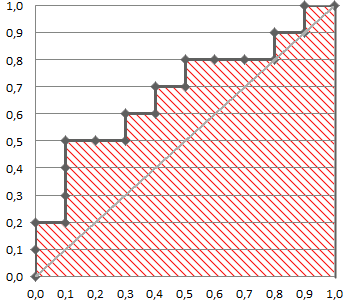
\includegraphics[width=0.38\textwidth]{figure_man/roc-auc-ex1.png}\hspace*{\fill}
%<!-- https://www.quora.com/How-is-statistical-significance-determined-for-ROC-curves-and-AUC-values -->
  % \item related to the Gini coefficient $= 2 \cdot AUC - 1$ (area above diag.)


\begin{vbframe}{Relation: AUC and Mann-Whitney-U test}
The AUC is the probability of a classifier ranking a randomly drawn positive observation higher than a randomly drawn negative one.
It is also related to the \textbf{Mann-Whitney-U test}:

\begin{itemize}
  \item How do observations rank when both groups ($\np$ and $\nn$) are pooled together?
  \item If the groups were drawn from the same underlying distribution, we expect the ranking to be uniform.
  \item The Mann-Whitney-U statistic simply counts for each observation in one group the number of times its value is ranked higher than any observation in the other group (in case of ties, we count 0.5).
  %the number of times a positive sample is greater than a negative sample.
  %\item To calculate a probability, we need compute the total number of ways the data will rank and compare to our observed ranking of the data.
\end{itemize}
% Source: https://medium.com/building-ibotta/understanding-roc-auc-part-2-2-a1e418a3afdb

\framebreak

\begin{itemize}
\item First we plot the ranks of all scores as a stack of horizontal bars and color them by label.
\item Stack the green bars on top of one another, and slide them horizontally as needed to get a nice, even stairstep on the right edge (see: practical method example for ROC curves):
\end{itemize}
\begin{center}
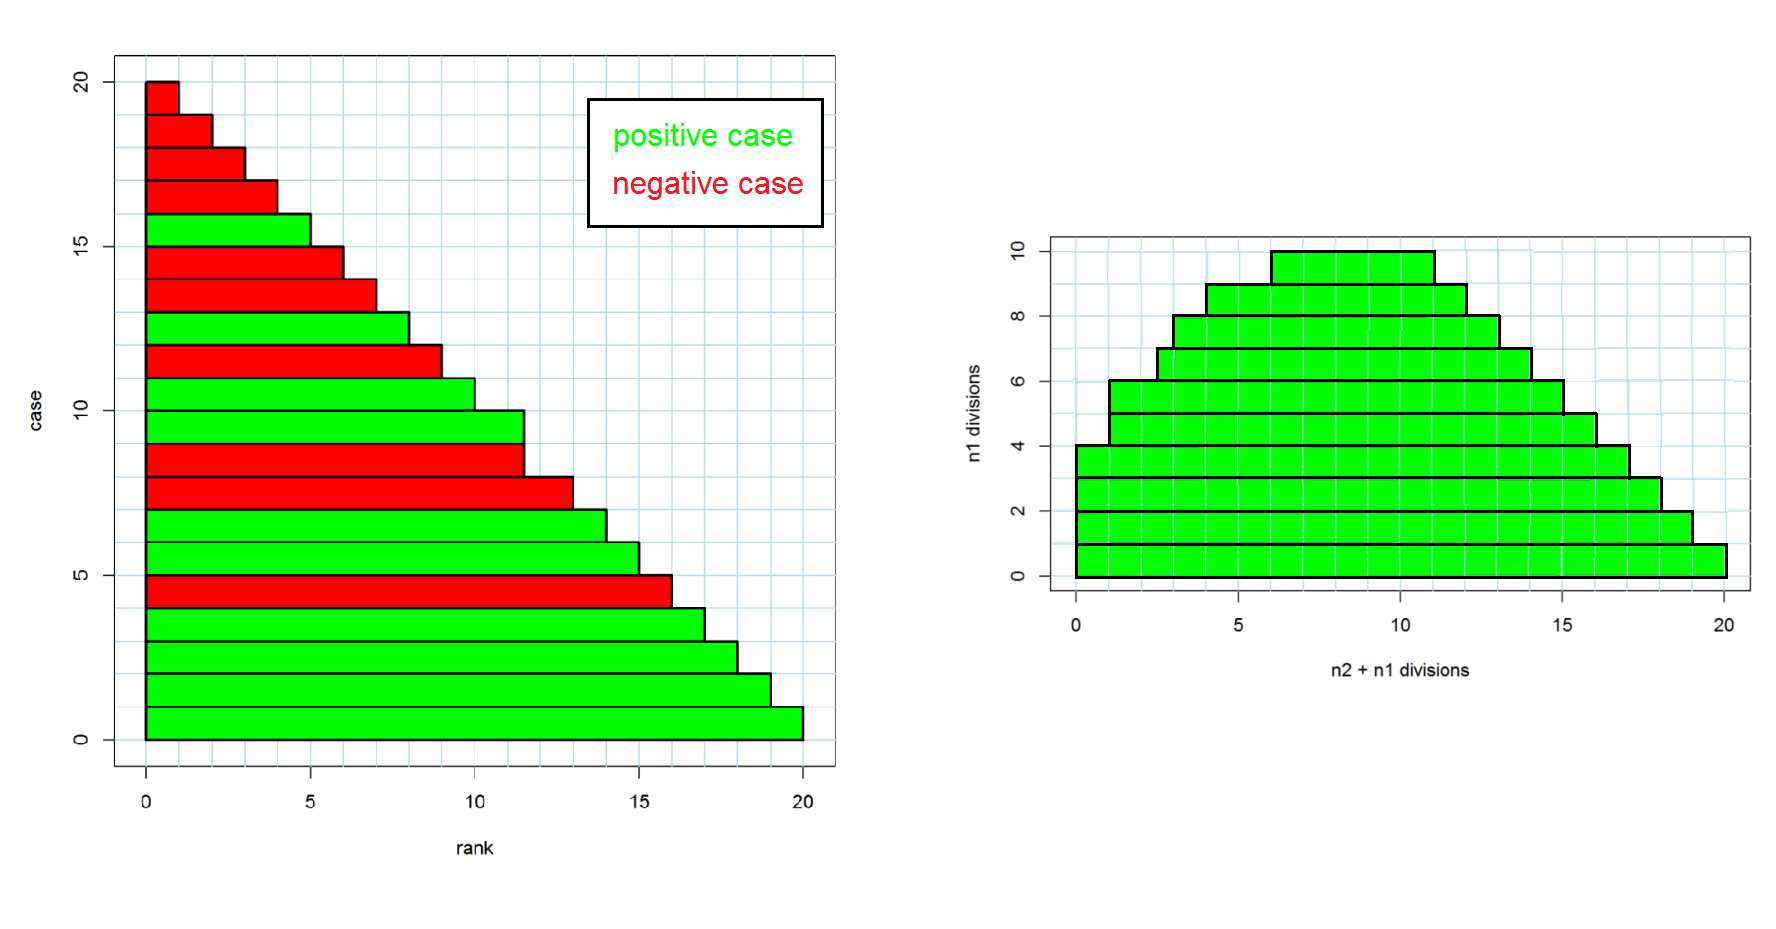
\includegraphics[width=0.8\textwidth]{figure_man/roc-mannwhitney3.png}
\end{center}


\framebreak


\begin{center}
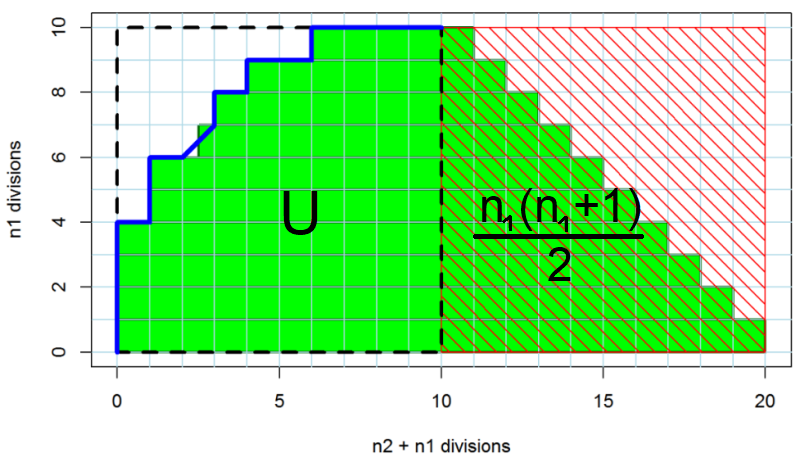
\includegraphics[width=0.5\textwidth]{figure_man/roc-mannwhitney2.png}
\end{center}

%\vspace{-15pt}
The sum of ranks of a sample of size $n$ is $\sum_{i=1}^{n} i = \frac{n(n+1)}{2}$.
We focus on the ranks of the group with size $n_1$:

\begin{itemize}
 \item Definition of the U statistic: $U = R_1 - \cfrac{n_1(n_1 + 1)}{2}$
 \begin{itemize}
  \item $R_1$ is the sum of ranks of positive samples, i.e., the area of all green bars.
  \item $n_1$ is the number of positive samples.
 \end{itemize}
  \item The area of the green bars on the right side is equal to $\cfrac{n_1(n_1 + 1)}{2}$.
\end{itemize}

\framebreak
\begin{center}
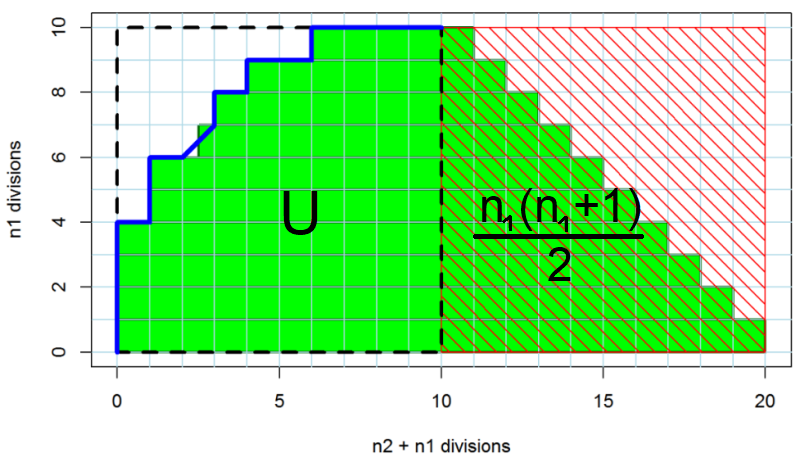
\includegraphics[width=0.5\textwidth]{figure_man/roc-mannwhitney2.png}
\end{center}

\begin{itemize}
 \item $U:$ area of the green bars on left side (if all positive samples ranked higher than the negative samples, we would have a green square on the left with $U = n_1 \cdot n_2$).
 \item $n_1 \cdot n_2:$ area of dashed rectangle on the left side.
 \item $AUC$ is $U$ normalized to the unit square, i.e.,
\end{itemize}
$$ AUC = \cfrac{U}{n_1\cdot n_2}$$
with $n_1 = \np$ and $n_2 = \nn$.
\end{vbframe}

\begin{vbframe}{Multiclass AUC}
\begin{itemize}
  \item Consider multiclass classification, where a classifier predicts the probability $p_g$ of belonging to class $g$ for each class.
  \item Hand and Till (2001)\footnote{Hand, D. J., Till, R. J. (2001). A simple generalisation of the area under the ROC curve for multiple class classification problems.} proposed to average the AUC of pairwise comparisons (\textbf{1-vs-1}) of a multiclass classifier:
  \begin{itemize}
    \item Estimate $AUC(i,j)$ for each pair of class $i$ and $j$.
    \item $AUC(i,j)$ is the probability of a randomly drawn member from class $i$ having a lower probability of belonging to class $j$ than a randomly drawn member of class $j$.
    \item For $g$ classes, we have ${{g}\choose{2}} = \tfrac{g (g-1)}{2}$ values of $AUC(i,j)$ that are then averaged to compute the multiclass AUC.
  \end{itemize}
\end{itemize}
\end{vbframe}


\begin{vbframe}{Multiclass AUC}
\begin{itemize}
  \item Provost and Domingos (2003)\footnote{Provost, F., Domingos, P. (2003). Tree induction for probability-based ranking.} proposed to average the AUC of \\
  \textbf{1-vs-rest} comparisons of a multiclass classifier.
  \item The idea is to iteratively take each class as the reference class, i.e., set the current class to 0 and all other classes to 1.
  \item Then average these single $AUC(i,j)$ values to compute the multiclass AUC according to \textbf{1-vs-rest}.
  \item For $g$ classes, we have $g$ values of $AUC(i,j)$ that are then averaged to compute the multiclass AUC.
\end{itemize}

\textbf{Note}: Both versions of the multiclass AUC can be weighted with their respective prior class distributions to also consider imbalanced classes.

% Source: https://link.springer.com/content/pdf/10.1023/A:1024099825458.pdf
\end{vbframe}


\begin{vbframe}{Multiclass AUC}

\begin{itemize}
  \item Note that the 1-vs-1 procedure is computationally heavier than 1-vs-rest.
  \item The 1-vs-rest approach leads to a skewed comparison as we create an artificial class imbalance even if the original classes were balanced in the first
  place.
  \item Provost and Domingos (2003) tried to solve the imbalance problem by
  incorporating the respective prior class distributions as weights.
\end{itemize}
\end{vbframe}


\endlecture
\end{document}
